\section{Introduction} \label{sec:introduction}
    \IEEEPARstart{R}{espiratory} motion reduces image resolution in \gls{PET} by introducing blurring \& mis-alignment artefacts~\cite{Nehmeh2008a}. Unless gated \gls{CT} are available (which themselves increase dose to the patient), to avoid mis-registration due to attenuation mismatches, most existing \gls{MC} methods rely on pair-wise registration of gated \gls{NAC} \gls{PET} volumes~\cite{LungMotionDiaphragmBaiBib}.%~\cite{Oliveira2014}.
    This is a challenging problem due to the low contrast \& high noise of these volumes. Other \gls{MC} methods can incorporate, directly, both \gls{MC} \& \glss{Mu-Map} estimation into reconstruction, however, these can be computationally expensive~\cite{Bousse2016b}.
    
    One \gls{MM} method uses \gls{3D} B-spline \gls{CPG} with the corresponding warping operation denoted as $\mathbf{W}(\mathbf{\alpha}_t)$, with $\mathbf{\alpha}_t$ a vector with coefficients at time $t$ \& the breathing surrogate signal $\mathbf{s}$:
    
    \begin{equation}
        \forall t \in [1, n_t],\quad \alpha_{k, t} := R_{1, k} s_{1, t} + R_{2, k}
    \end{equation}
    
    \noindent where $\alpha_{k, t}$ is the coefficient for node $k$ at time point $t$, \& $R_{i, k}$ are the model parameters where $i = [1, 2]$~\cite{McClelland2017}. One of the advantages of using a \gls{MM} approach over registering all the data to a static volume is that by incorporating a fit on the \gls{SS} noise from outlying registrations is diminished.
    
    In our previous work we investigated the possibility of using \gls{MM} for respiratory \gls{MC} where the \gls{RCM} was derived from \gls{NAC} \gls{PET}. We found that \gls{NAC} \gls{TOF} \gls{PET} was suitable to estimate the motion from gated PET data without inter-respiratory cycle variation~\cite{Whitehead2019ImpactPET}. This work extends the method towards \gls{AC} with a single \gls{Mu-Map} (from any position).

\section{Methods} \label{sec:methods}
    \subsection{XCAT Volume Generation} \label{sec:xcat_volume_generation}
        \gls{XCAT}%~\cite{Segars2010}
        was used to generate $240$ volumes over a \SI{120}{\second} respiratory trace (with inter-respiratory cycle variation) derived from a respiratory trace captured using a \gls{RPM}. The max displacement of \gls{AP} \& \gls{SI} motion was set to \SI{1.2}{\centi\metre} \& \SI{2.0}{\centi\metre} respectively. Activity concentrations were derived from a static \gls{FDG} patient scan. The \gls{FOV} included the base of the lungs, diaphragm \& the top of the liver with a \SI{20}{\milli\metre} diameter spherical lesion placed into the centre of the right lung.
    
    \subsection{PET Acquisition Simulation} \label{sec:pet_acquisition_simulation}
        \gls{PET} acquisitions were simulated %(and reconstructed)
        using \gls{STIR}~\cite{Thielemans2012, Efthimiou2018} through \gls{SIRF}~\cite{ Ovtchinnikov2019CCPPETMRSIRF} to forward project the data using the geometry of a \gls{GE} Discovery $710$ with a \gls{TOF} resolution of \SI{375}{\pico\second}. This \gls{TOF} resolution is higher than that of the \gls{GE} Discovery 710, but is closer to the newer \gls{GE} Signa \gls{PET}/\gls{MR} system. \gls{TOF} mashing is used to reduce computation time resulting in $13$ \gls{TOF} time bins of size \SI{376.5}{\pico\second}. Attenuation was included using the relevant \glss{Mu-Map} generated by \gls{XCAT}. Scatter \& randoms were not taken into account. Multiple noise realisations were generated to simulate an acquisition over \SI{120}{\second}, emulating a standard single bed position acquisition. A respiratory \gls{SS} was generated using \gls{PCA}.%~\cite{Thielemans2011}.
        This was used to gate the data into $10$ respiratory bins using displacement gating.% For the purpose of the \gls{RCM} fitting, \gls{SS} values were ascertained for the post-gated data by taking an average of the \gls{SS} values of the data in each bin.
    
    \subsection{Non-Attenuation Corrected Image Reconstruction} \label{sec:non-attenuation_corrected_image_reconstruction}
        Data were reconstructed without \gls{AC} using \gls{OSEM} with two full iterations \& $24$ subsets.%~\cite{Hudson1994}.
        Volumes were post-filtered using a Gaussian blur with a kernel size of \SI{6.4}{\milli\metre} \gls{FWHM}.
    
    \subsection{Motion Model Estimation} \label{sec:motion_model_estimation}
        For each dataset \gls{3D} B-spline interpolated \glss{CPG} were used to model spatial deformations. A generalised framework unifying \gls{IR} \& respiratory \glss{MM} was used to estimate \glss{RCM} \& \glss{MCIR}~\cite{McClelland2017}. \gls{SSD} was used as the similarity measure \& bending energy was used as a penalty.% The \gls{CPG} spacing \& penalty weight were tuned using a grid search.
    
    \subsection{Attenuation Map Warping} \label{sec:attenuation_map_warping}
        A \gls{Mu-Map}, as close to the mean respiratory position as possible, was selected from the \glss{Mu-Map} generated by \gls{XCAT}, this \gls{Mu-Map} was then registered to the mean position volume generated while fitting the \gls{RCM} from~\Fref{sec:motion_model_estimation}. A \gls{NMI} registration was used to accomplish this.% with parameters selected using a grid search.
        The \gls{RCM} was then used to generate \glss{DVF} for the \gls{SS} values of each bin, which were then used to warp the \gls{Mu-Map} from the mean respiratory position to each bin.
        
    \subsection{Attenuation Corrected Motion Corrected Image Reconstruction} \label{sec:attenuation_corrected_image_reconstruction}
        Data were re-reconstructed with \gls{AC} using the \glss{Mu-Map} from~\Fref{sec:attenuation_map_warping}. The same reconstruction parameters as in~\Fref{sec:attenuation_corrected_image_reconstruction} were used. This data was then either \gls{MC} using the original \gls{NAC} \gls{RCM} or a new \gls{RCM} was fit on the \gls{AC} data as in~\Fref{sec:motion_model_estimation}.
    
    \subsection{Evaluation} \label{sec:evaluation}
        %To evaluate the validity of the \gls{MM} results, the \gls{COM} of the lesion, over time, was tracked for both \gls{NAC} \& \gls{AC} reconstructions. This was achieved by warping a volume only including the lesion in the reference position, \& then computing its \gls{COM}.
        
        In addition to the reconstructions performed in~\Fref{sec:attenuation_corrected_image_reconstruction} data were also reconstructed by simply summing all gates together \& using either a sum of all \glss{Mu-Map} (to emulate a \gls{CCT}) or one \gls{Mu-Map}, positioned as close to the mean respiratory position as possible, for \gls{AC}, this process matches \gls{CCP}. The data from this approach was used to evaluate the improvement that the new method afforded. The comparisons used included: a visual analysis, a profile over the lesion \& \gls{SUV}\textsubscript{max}, \gls{SUV}\textsubscript{median} \& \gls{SUV}\textsubscript{peak}. \gls{SUV}\textsubscript{peak} here was defined following \gls{EANM} guidelines.%~\cite{Boellaard2015FDG2.0}

\section{Results} \label{sec:results}
    %\begin{figure}
    %    \centering
    %    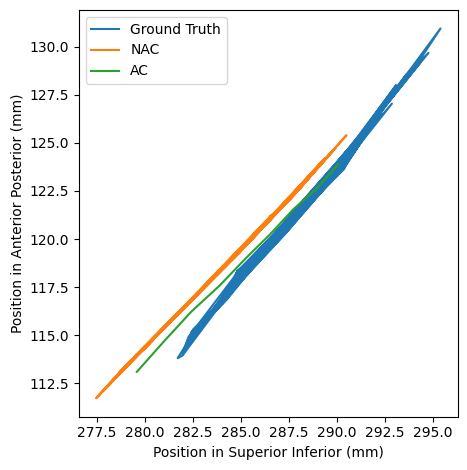
\includegraphics[width=0.5\linewidth]{figures/com.png}
    %    \captionsetup{singlelinecheck=false, justification=centering}
    %    \caption{The path of the \gls{COM} of the lesion. Horizontal (respectively vertical) axis corresponds to motion in the \gls{SI} (respectively \gls{AP}). Different curves denote \gls{COM} displacement for  ground truth data, the estimated data from the \gls{NAC} based \gls{RCM} \& the estimated data from the \gls{AC} based \gls{RCM}.}
    %    \label{fig:com}
    %\end{figure}
    
    %\gls{COM} results can be seen in~\Fref{fig:com}, the \gls{COM} of both the \gls{NAC} \& \gls{AC} matches closely the ground truth \gls{COM}.
    
    \begin{figure}
        \centering
        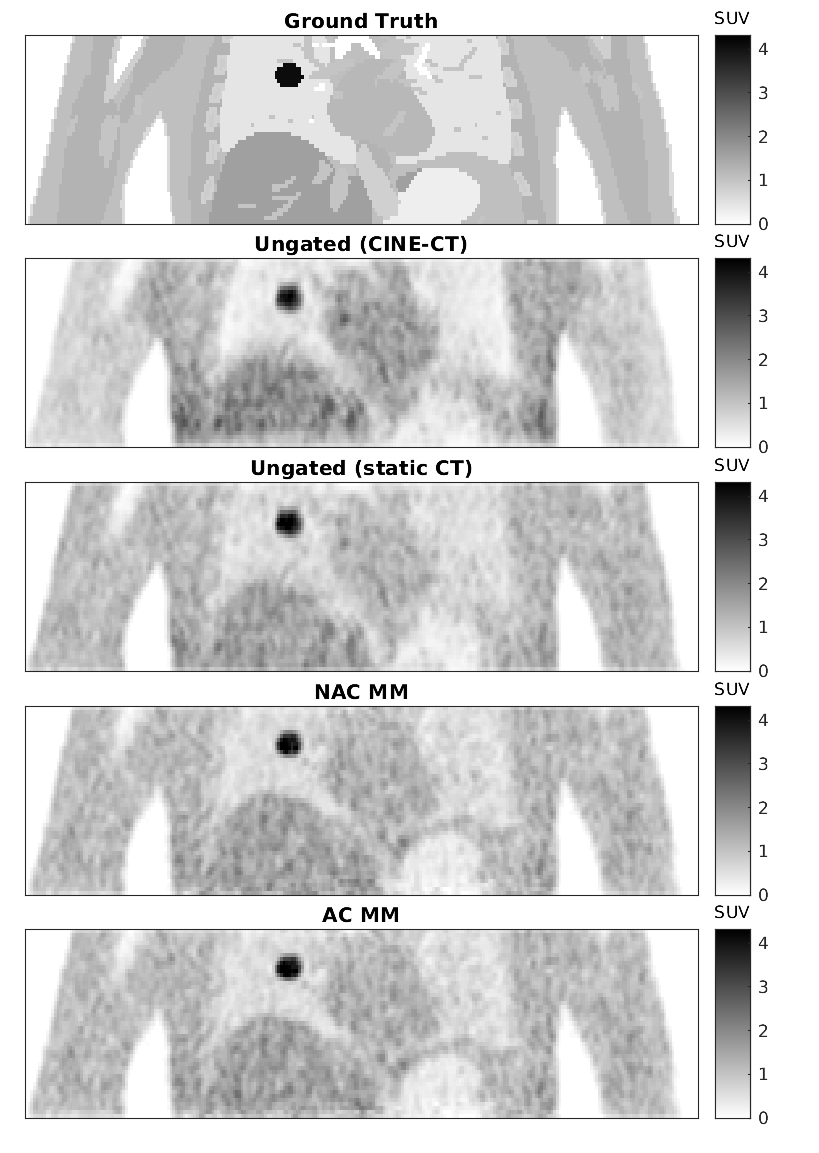
\includegraphics[width=0.75\linewidth]{figures/visual_analysis.png}
        \captionsetup{singlelinecheck=false, justification=centering}
        \caption{First row: \gls{CCP} using a \gls{CCT} \gls{Mu-Map}. Second row: \gls{CCP} using a static \gls{CT} \gls{Mu-Map}. Third row: New method using the \gls{NAC} \gls{RCM}. Forth row: New method using the \gls{AC} \gls{RCM}. Colour map ranges are consistent for all images.}
        \label{fig:visual_analysis}
    \end{figure}
    
    \begin{figure}
        \centering
        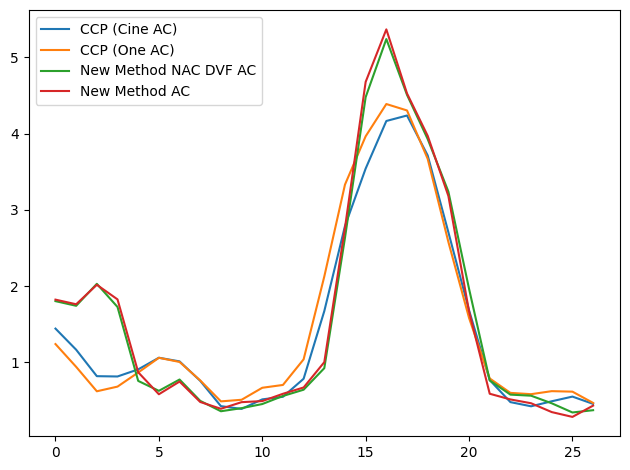
\includegraphics[width=0.5\linewidth]{figures/profile.png}
        \captionsetup{singlelinecheck=false, justification=centering}
        \caption{A profile across the lesion for the \gls{CCP} using a \gls{CCT} \gls{Mu-Map} volume, \gls{CCP} using a static \gls{CT} \gls{Mu-Map} volume, new method using the \gls{NAC} \gls{RCM} volume \& new method using the \gls{AC} \gls{RCM} volume.}
        \label{fig:profile}
    \end{figure}
    
    \begin{table}
        \centering
        \captionsetup{singlelinecheck=false, justification=centering}
        \caption{Comparison of \gls{SUV}\textsubscript{max}, \gls{SUV}\textsubscript{median} \& \gls{SUV}\textsubscript{peak} between the \gls{CCP} using a \gls{CCT} \gls{Mu-Map} volume, \gls{CCP} using a static \gls{CT} \gls{Mu-Map} volume, new method using the \gls{NAC} \gls{RCM} volume \& new method using the \gls{AC} \gls{RCM} volume.}
        
        \resizebox*{0.75\linewidth}{!}
        {
            \begin{tabular}{||c|ccc||}
                \hline
                \textbf{\gls{SUV}} & \textbf{Max} & \textbf{Median} & \textbf{Peak} \\
                \hline
                \textbf{\gls{CCP} (\gls{CCT})}          & $4.63$ & $2.73$ & $3.39$ \\
                \textbf{\gls{CCP} (One \gls{CT})}       & $4.66$ & $3.05$ & $3.54$ \\
                \hline
                \textbf{New Method \gls{NAC} \gls{DVF}} & $5.56$ & $3.18$ & $4.07$ \\
                \textbf{New Method \gls{AC} \gls{DVF}}  & $5.43$ & $3.18$ & $4.00$ \\
                \hline
            \end{tabular}
        }
        \label{tab:suv}
    \end{table}
    
     The \gls{CCP} data \& the new method data can be seen in~\Fref{fig:visual_analysis}. When compared visually structures can be seen in the new method data that cannot be seen in the \gls{CCP} data, for instance, structures at the boundary between the diaphragm \& the lung. Additionally, the boundary between the lesion \& the lung appears to be sharper \& the lesion itself more homogeneous, this can be observed in the profile across the lesion in~\Fref{fig:profile}. \gls{SUV} results can be seen in~\Fref{tab:suv} \& consistently show that \glss{SUV} are greater for the new method over \gls{CCP}.

\section{Discussion \& Conclusions} \label{sec:discussion_and_conclusions}
    %\glss{MM} derived from \gls{NAC} \& \gls{AC} volumes for both data containing intra- \& inter-respiratory cycle motion were found to be relatively robust when comparing \gls{COM}. 
    Results from both a visual analysis \& from a comparison of profiles \& \glss{SUV} shows that the new method provides volumes more free from blurring \& less susceptible to artefacts when compared to \gls{CCP}.
    
    In the future, research will focus on more complex methods of incorporating, directly, both \gls{MC} \glss{Mu-Map} \& \gls{MM} into reconstruction.